\RequirePackage[l2tabu, orthodox]{nag}
\documentclass[12pt]{article}

\usepackage{amssymb,amsmath,verbatim,graphicx,microtype,upquote,units,booktabs,siunitx,xcolor,wrapfig,pgfplots,graphics}
\usepackage[margin=10pt, font=small, labelfont=bf, labelsep=endash]{caption}

\newcommand{\fundamental}[1]{\colorbox{gray!30}{\strut$#1$}}
\setlength\parindent{0pt}
\pgfplotsset{compat=newest}

\newcommand{\wave}{
    \begin{tikzpicture}[scale=0.1, transform shape]
    \begin{axis}[
      xmin=-15,
      xmax=15,
      ymin=-2,
      ymax=2,
      axis x line=middle,
      axis y line=middle,
      yticklabels={,,},
      xticklabels={,,},
      samples = 2000
    ]
    \addplot[red] {2*exp(-0.05*x^2)*cos(deg(3.5*x))};

    \end{axis}
    \end{tikzpicture}
}

\title{Modern Physics Review}
\date{\today}
\author{Illya Starikov}

\begin{document}
\maketitle




\section{Special Relativity}
From relativity, we know

\begin{enumerate}
    \item All inertial reference frames are equivalent.
    \item The speed of light is the same in all inertial reference frames.
\end{enumerate}

From this, we notice that

\begin{enumerate}
    \item Time and space depend on velocity ($\vec{v}$).
    \item Moving clocks appear to run slow.
    \item The length of a moving object, in the direction of motion, will appear shorter.
\end{enumerate}

Eloquently, this can be described as

\begin{equation*}
    \fundamental{t = \gamma t_0} \quad\quad \fundamental{L = \frac{L_0}{\gamma}}
\end{equation*}

Where \fundamental{\gamma = \frac{1}{\sqrt{1 - \nicefrac{v^2}{c^2}}}}, $t$ is the time according to the outside observer, $t_0$ to be proper time (i.e. the time measured by the moving object), $L$ is length to outside observer, and $L_0$ is proper length.


\section{Energy and Momentum}
Relativistic energy and momentum can be defined as

\begin{equation*}
    \fundamental{E = \gamma m_0 c^2} \quad\quad \fundamental{\vec{p} = \gamma m_0 \vec{v}}
\end{equation*}

From the this, we can derive the more fundamental equation:

\begin{equation}\label{eq:energy}
    E^2 = m_0^2 c^4 + p^2 c^2
\end{equation}

For kinetic energy, we can eloquently describe it as \fundamental{(\gamma - 1)m_0 c^2}, this is simply the rest mass energy ($mc^2$) subtracted from the total energy ($\gamma mc^2$). At low speeds (i.e. $v \ll c$), we can simply use a Taylor Series expansion to get $E \approx \nicefrac{1}{2} m_0 v^2 + \frac{3 m_0 v^4}{8c^2} + \cdots$. Ignoring the other terms, we get $E \approx \nicefrac{1}{2}m v^2$, classical energy!

If we take $m_0$ to be $0$, this implies $E = pc$ (From Equation \ref{eq:energy}). Using de Broglie wavelength (\fundamental{\lambda = \nicefrac{h}{p}}), this is implies \fundamental{E = h\nu}. This can be combined with the fact that \fundamental{\lambda \nu = c}, which allows many permutations of the equations. We can also show that the kinetic energy \fundamental{KE = \frac{p^2}{2m}} To summarize, for $m_0 = 0$,

\begin{equation*}
    E = h\nu = \frac{hc}{\lambda} = pc
\end{equation*}


\section{The Three Experiments}
\begin{wrapfigure}{r}{0.5\textwidth}
    \centering
    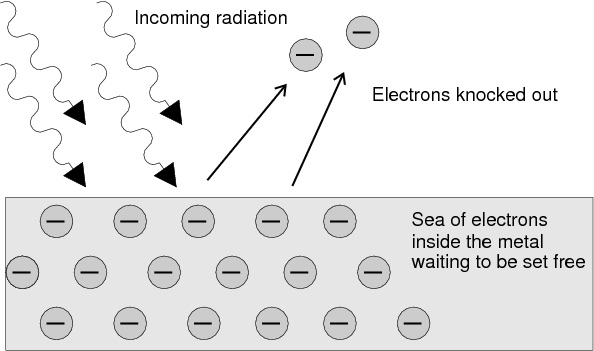
\includegraphics[width=.45\textwidth]{photo-electric-effect}

    \caption{The Photoelectric Effect.}
    \label{fig:photo-electric-effect}
\end{wrapfigure}

There were three experiments done to prove the quantum nature of light and particles.

\subsection{The Photoelectric Effect}
Suppose we have a sea of electrons within a metal. It takes some work to escape the sea, described by the work function $\Phi$. We can relate the energy of the photon, the work function, and the resulting energy of the electrons by $h \nu = \Phi + KE_{\text{max}}$.

\subsection{Compton Scattering}
We can scatter a photon off an electron, inelastically, and after some tedious math we can realize $\lambda_2 - \lambda_1 = \frac{h}{m_0 c}(1 - \cos\theta)$, where $\lambda_2$ is the wavelength after scattering, $\lambda_1$ is the wavelength before the scattering, and $m_0$ the electron rest mass. From this we realize that there is a decrease in the energy of the photon, resulting in an increase of wavelength, which we know as the Compton effect.

\begin{figure}[!ht]
    \centering
    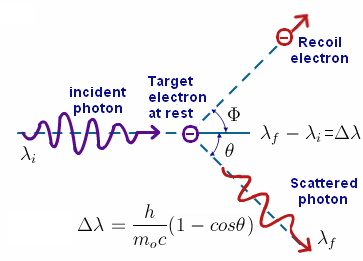
\includegraphics[width=.45\textwidth]{compton-scattering}

    \caption{Compton scattering.}
    \label{fig:compton-scattering}
\end{figure}

\subsection{Blackbody Radiation}
Blackbody radiation refers to an object or system which absorbs all radiation incident upon it and re-radiates it.
This effect can be characterized by the radiating system alone; it does not depend on the type of radiation incident upon it.
The radiated energy can be considered to be produced by standing wave or resonant modes of the cavity which is radiating. The major effect of this is that the modes must be quantized. We can define the energy per unit volume per unit frequency

\begin{equation*}
    U(\nu) = \frac{8 \pi \nu^2}{c^3} \frac{h \nu}{e^\frac{h \nu}{kT} - 1}
\end{equation*}

where $k$ is the Boltzmann constant and $T$ is the absolute temperature of the body. The entity $\frac{h \nu}{e^{\nicefrac{h \nu}{kT}} - 1}$  is the average energy per mode, and $\frac{8 \pi \nu^2}{c^3}$ counts the number of modes available.


\section{Wave Nature of Massive Particles}
% We recall that \fundamental{p = \nicefrac{h}{\lambda}} and \fundamental{E = h\nu}, which \textit{is true for all particles}, massive or not. The wavelength implies there to be a wavefunction $\psi(x)$ (\wave), where the wavefunction tells us what the wave is. With a known wavefunction, we can tell the probability of finding where the particle.

\begin{align*}
    |\psi (x)|^2 dx = &\text{ the probability of finding the} \\
                      &\text{ particle in the range of $x$ to $x+dx$}
\end{align*}

Because $|\psi(x)|^2$ is a continuous probability distribution, we must normalize the wavefunction so that the probability has to add up to $100\%$,

\begin{equation*}
    \int _{-\infty} ^{\infty} |\psi(x)|^2 \, dx = 1
\end{equation*}

\subsection{Uncertainty Principle}
It can be derived that for an particular measurement,

\begin{equation*}
    \Delta t \Delta E \geq \frac{\hslash}{2} \quad\quad \hslash = \frac{h}{2\pi}
\end{equation*}

Or, more famously,

\begin{equation*}
    \Delta x \Delta p \geq \frac{\hslash}{2} \quad\quad \hslash = \frac{h}{2\pi}
\end{equation*}

\subsection{Infinite Potential Well}

\begin{wrapfigure}{r}{0.5\textwidth}
    \centering
    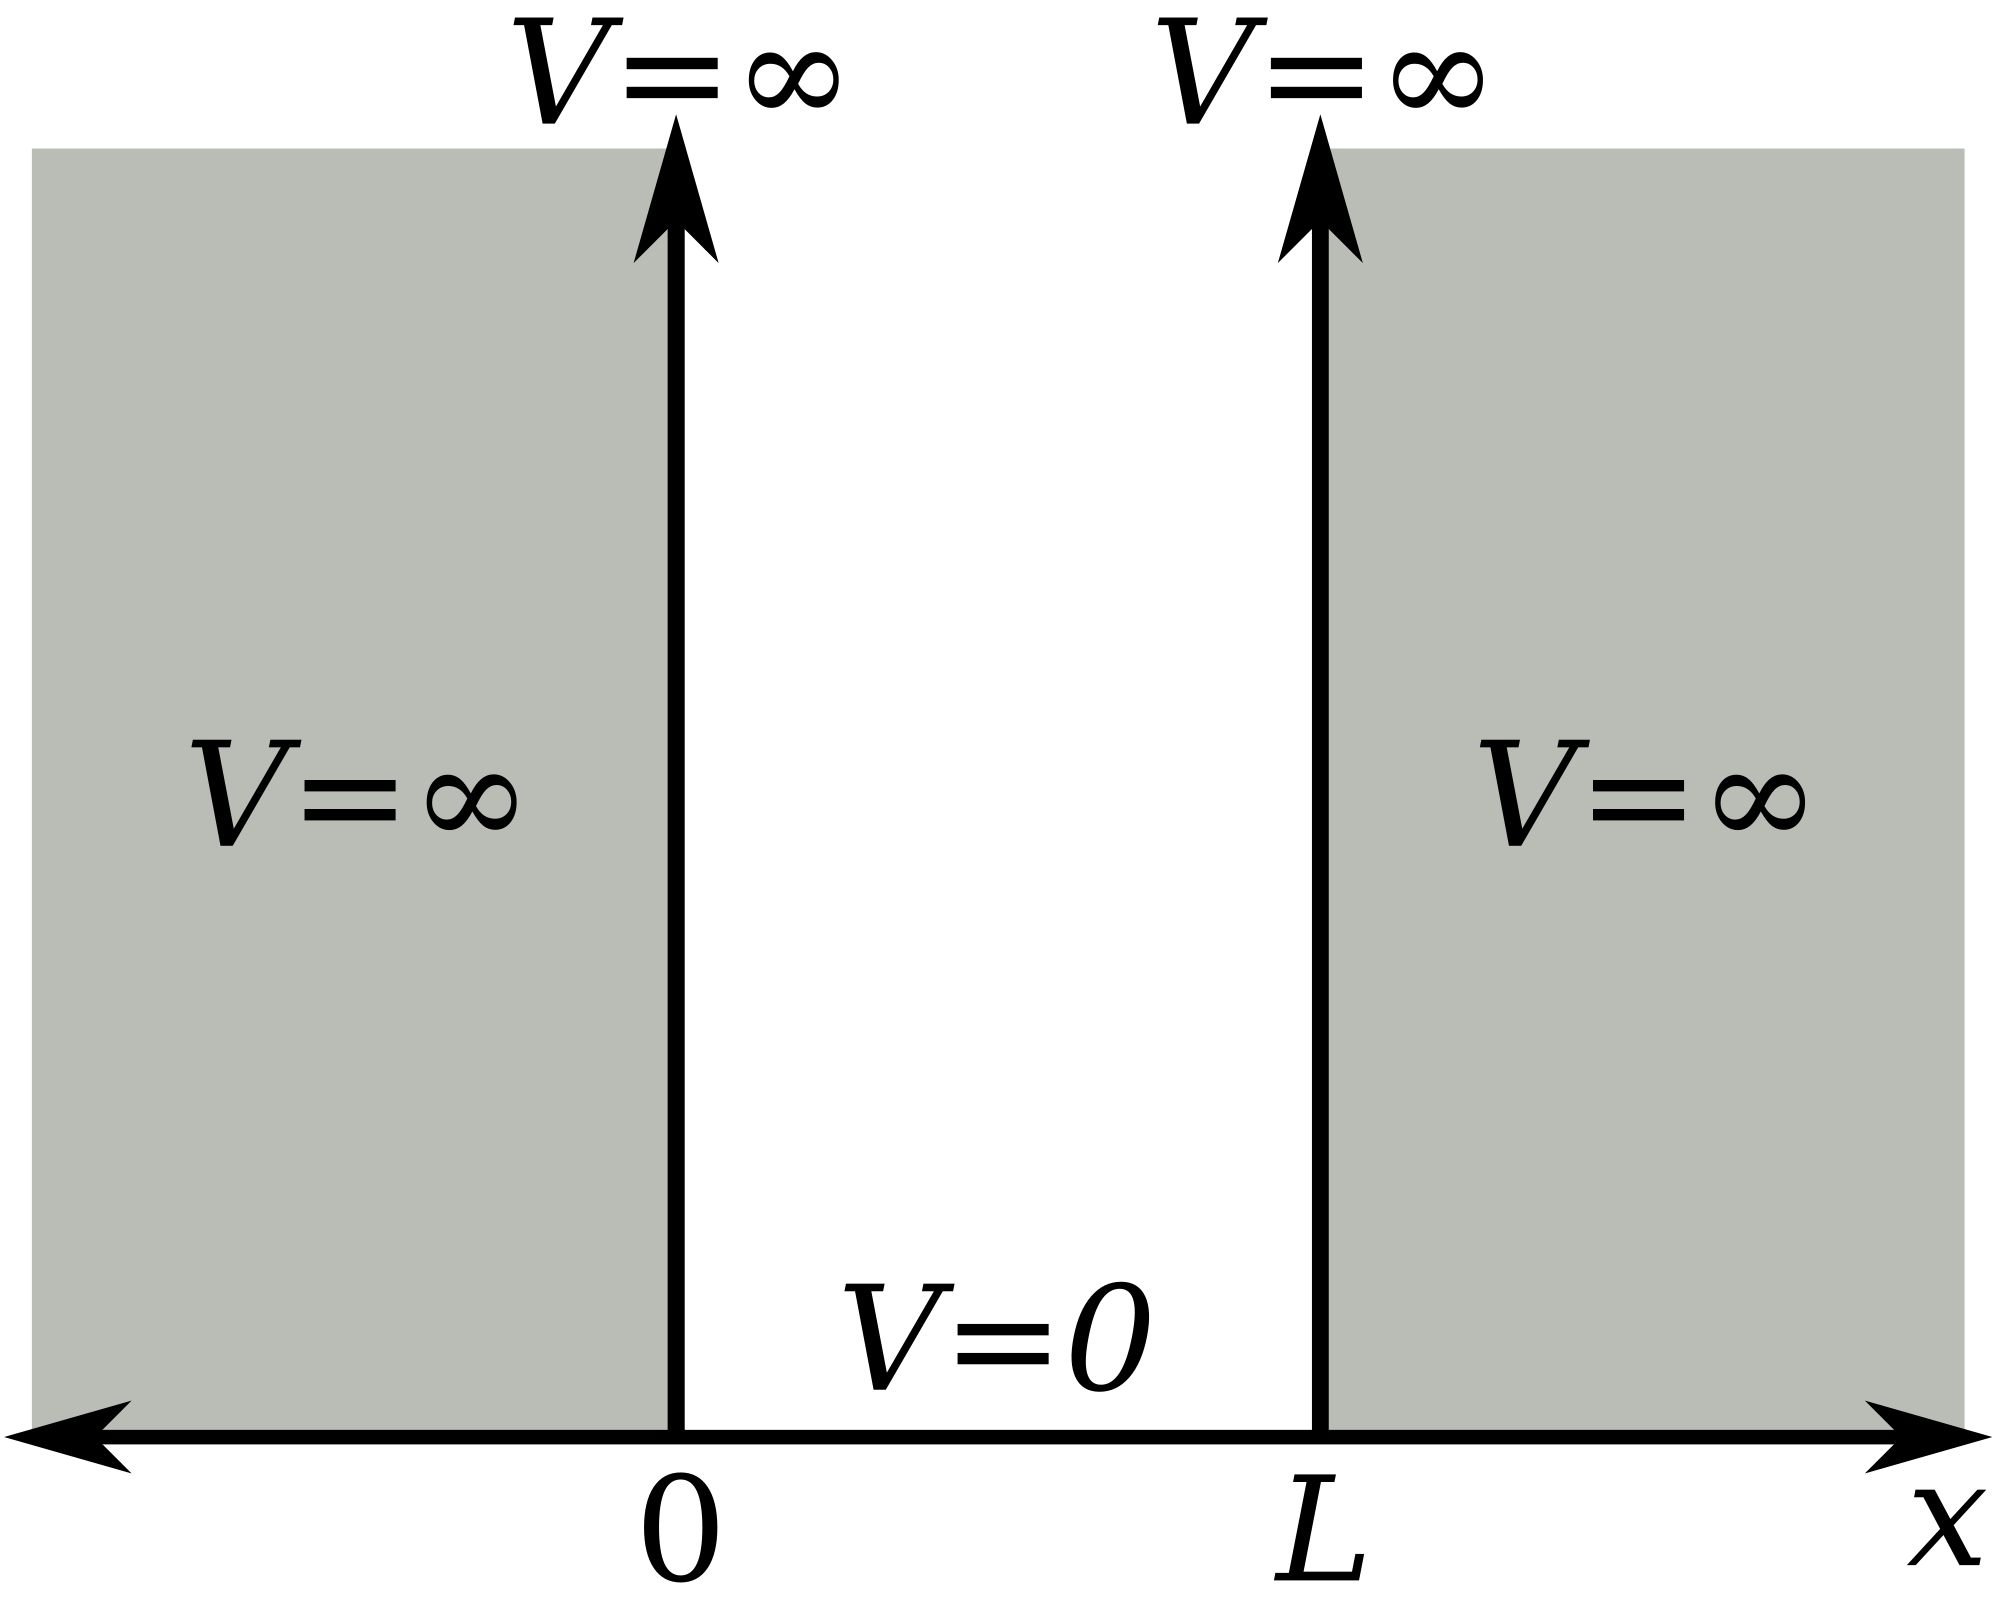
\includegraphics[width=.45\textwidth]{particle-in-a-box}

    \caption{Particle in a box (or infinite potential well).}
    \label{fig:potential-well}
\end{wrapfigure}

Imagine a potential wall where the wall go to infinity, with a distance $L$ between the walls. Our wave function $\psi$ must have the boundary conditions $\psi(x=0) = 0$ and $\psi(x=L) = 0$. From this we realize we can only fit half-wavelengths of the wave into the box; that is, $n \nicefrac{\lambda}{2} = L$. To calculate the energy,

\begin{align*}
    \fundamental{E = \frac{p^2}{2m} = \frac{n^2 h^2}{8mL^2}}
\end{align*}

because $\lambda = \frac{2L}{n}$ and $p = \frac{h}{\lambda}$.

\subsection{Wave Motion}
We know we can describe just about any wave by $\cos(kx - \omega t)$, where $k = \frac{2\pi}{\lambda}$ and $\omega = 2\pi\nu$. Consequently, $p = \nicefrac{h}{\lambda} = \hslash k$ and $E = h\nu = \hslash\omega$.

Furthering our wave mathematics, we can consider the phase velocity as

\begin{equation*}
    v_p = \frac{\omega}{k} = \frac{E}{p} = \nu\lambda
\end{equation*}

When considering a group, we can calculate the velocity of the group (or the packet), $v_g$, as

\begin{equation*}
    v_g = \frac{\partial \omega}{\partial k} = \frac{\partial E}{\partial p}
\end{equation*}

\subsection{Hydrogen Atom}
As we have proven with our three experiments, energy states are quantized. This implies that the energy levels in an atom come in integer levels (i.e. energy level $n = 1, 2, 3, \ldots, \infty$, where $\infty$ is ionization).

\begin{wrapfigure}{l}{0.5\textwidth}
    \centering
    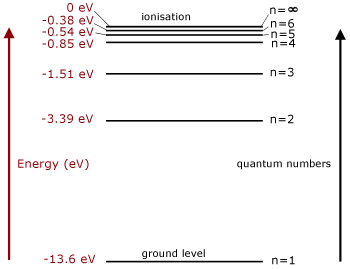
\includegraphics[width=.45\textwidth]{energy-levels}

    \caption{Energy levels of hydrogen atom.}
    \label{fig:energy-levels}
\end{wrapfigure}

From this, we can determine that the energy at any level $E_n = \frac{E_1}{n^2}$, where $E_1 < 0$. For photo-absorption,

\begin{align*}
    h\nu = E_f - E_i &= \frac{E_1}{n_f ^2} - \frac{E_1}{n_i ^2} \\
                                  &= \fundamental{E\left( \frac{1}{n_f ^2} - \frac{1}{n_i ^2} \right)}
\end{align*}

Similarly, for emission,

\begin{align*}
    h\nu = E_i - E_f &= \frac{E_1}{n_i ^2} - \frac{E_1}{n_f ^2} \\
                                  &= \fundamental{E\left( \frac{1}{n_i ^2} - \frac{1}{n_f ^2} \right)}
\end{align*}



\end{document}
